\section*{Introduction}

PBDataAnalysis is a C library providing structures and functions to perform various data analysis.\\ 

It implements the following algorithms:
\begin{itemize}
\item K-means clustering (random and Forgy seeds)
\end{itemize}

It uses the \begin{ttfamily}PBErr\end{ttfamily}, \begin{ttfamily}PBMath\end{ttfamily}, \begin{ttfamily}GSet\end{ttfamily} libraries.\\

\section{Definitions}

\subsection{K-means clustering}

The goal of the K-means clustering algorithm is to find K Voronoi cells which clusters a data set in a way that for each cells the center of this cell is the nearest possible to the average value of the input data inside this cell.\\

The K-means algorithm is as follow, where 'seed' defines the way we initialise the algorithm: 'random' or 'Forgy'.\\

\begin{scriptsize}
\begin{ttfamily}
\verbatiminput{/home/bayashi/GitHub/PBDataAnalysis/Doc/kmeansclustering.txt}
\end{ttfamily}
\end{scriptsize}

\section{Interface}

\begin{scriptsize}
\begin{ttfamily}
\verbatiminput{/home/bayashi/GitHub/PBDataAnalysis/pbdataanalysis.h}
\end{ttfamily}
\end{scriptsize}

\section{Code}

\subsection{pbdataanalysis.c}

\begin{scriptsize}
\begin{ttfamily}
\verbatiminput{/home/bayashi/GitHub/PBDataAnalysis/pbdataanalysis.c}
\end{ttfamily}
\end{scriptsize}

\section{Makefile}

\begin{scriptsize}
\begin{ttfamily}
\verbatiminput{/home/bayashi/GitHub/PBDataAnalysis/Makefile}
\end{ttfamily}
\end{scriptsize}

\section{Unit tests}

\begin{scriptsize}
\begin{ttfamily}
\verbatiminput{/home/bayashi/GitHub/PBDataAnalysis/main.c}
\end{ttfamily}
\end{scriptsize}

\section{Unit tests output}

\begin{scriptsize}
\begin{ttfamily}
\verbatiminput{/home/bayashi/GitHub/PBDataAnalysis/unitTestRef.txt}
\end{ttfamily}
\end{scriptsize}

kmeancluster.csv:\\
\begin{scriptsize}
\begin{ttfamily}
\verbatiminput{/home/bayashi/GitHub/PBDataAnalysis/kmeancluster.csv}
\end{ttfamily}
\end{scriptsize}

random seed in grey, Forgy seed in black:\\
\begin{center}
\begin{figure}[H]
\centering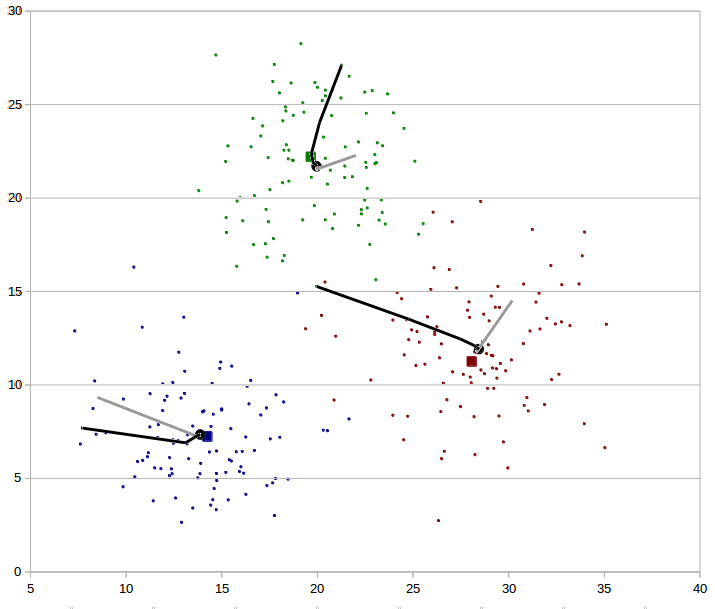
\includegraphics[width=6cm]{./kmeansclustering.png}\\
\end{figure}
\end{center}
